\subsection{Voraussetzungen}
Für die Entwicklung werden folgende Rahmenbedingungen empfohlen:
\begin{itemize}
  \item \textbf{Betriebssystem:} Linux (primär getestet unter Arch Linux).
\item \textbf{Shell/Terminal:} Keine feste Shell-Vorgabe. Die Projektsteuerung erfolgt über  \textbf{Python-Skripte}; eine interaktive Shell wird lediglich zum Aufruf der Befehle benötigt.
  \item \textbf{Zugriffsrechte:} Installation von Paketen/Toolchains (je nach System via Paketmanager).
  \item \textbf{Versionsverwaltung:} Git.
\end{itemize}

\subsubsection{Layer-Modell der Entwicklungsumgebung}

Zur besseren Einordnung der eingesetzten Werkzeuge lässt sich die Entwicklungsumgebung in funktionale Layer gliedern. Diese Layer beschreiben nicht die Programmarchitektur, sondern die Umgebung, in der Entwicklung, Build und Ausführung stattfinden.

\begin{itemize}
  \item \textbf{Basissystem (System Layer)} \\
  Betriebssystem und grundlegende Systemdienste (Linux, macOS, Windows) bilden die technische Basis. In diesem Layer befinden sich außerdem systemweite Werkzeuge wie Git, Compiler, Paketmanager und Laufzeitumgebungen.

  \item \textbf{Automatisierungs- und Skript-Layer} \\
  Installations-, Diagnose- und Steuerungslogik ist plattformübergreifend in \textbf{Python} implementiert. Dieser Layer kapselt wiederkehrende Aufgaben wie Setup, Dependency-Prüfung, Build und Start des Projekts und abstrahiert Plattformunterschiede.

  \item \textbf{Tool- und Framework-Layer} \\
  Entwicklungswerkzeuge und Frameworks wie Rust, Node.js, Tauri sowie der verwendete Paketmanager stellen die eigentliche Build- und Laufzeitumgebung für Backend und Frontend bereit.

  \item \textbf{Entwicklungs- und Prozess-Layer} \\
  IDEs (z.\,B. VS Code), Editor-Erweiterungen, Linter, Formatter und Dev-Server unterstützen den täglichen Entwicklungsprozess. Dieser Layer beeinflusst die Developer Experience, jedoch nicht das resultierende Programmverhalten.
\end{itemize}

Dieses Layer-Modell dient der strukturellen Einordnung der Entwicklungsumgebung und schafft eine klare Trennung zwischen Systembasis, Automatisierung, Toolchain und entwicklungsbegleitenden Prozessen.


\begin{figure}[H]
    \centering
    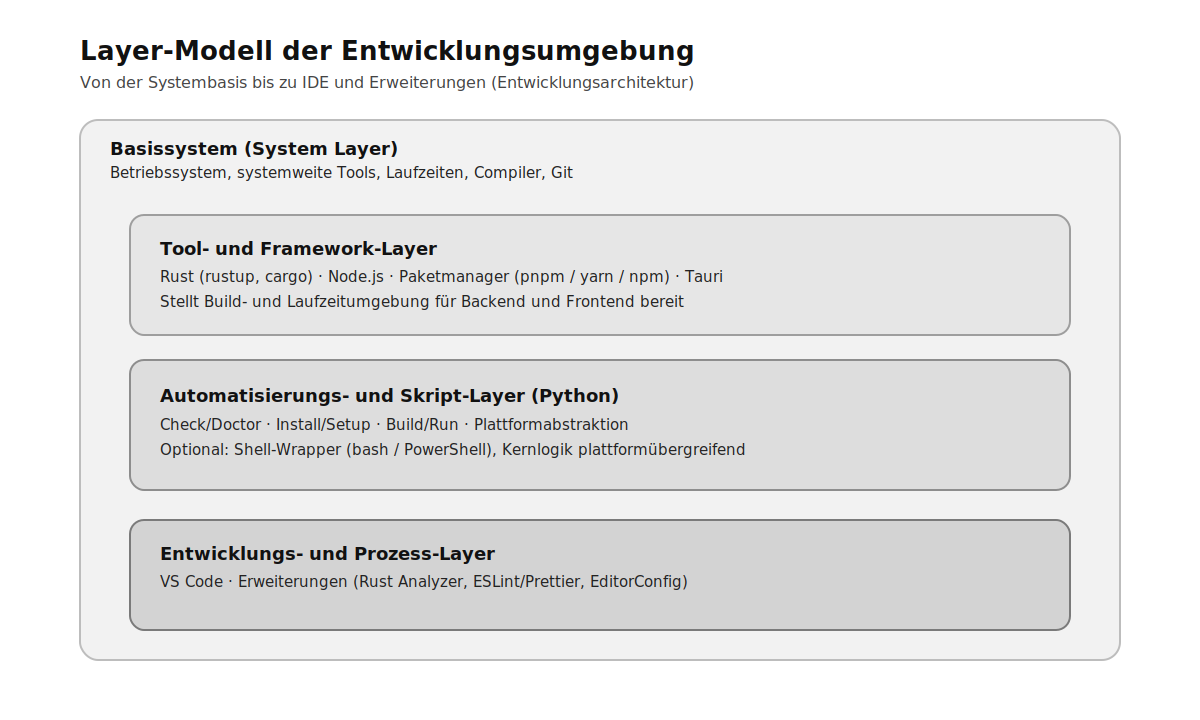
\includegraphics[width=0.95\textwidth]{FMD/image/LayerDevelopDE.png}
    \caption{Layer-Modell \projektname\ .\cite{Eigendarstellung}}
    \label{fig:zielsetzung-architektur}
\end{figure}

